\section{Gaussian Process Regression}
\label{gp}

Evaluating the production curve for a specific kind of facility using 
full fuel cycle simulations is relatively expensive, even in the 
computationally cheapest case. This is because a fuel cycle realization 
typically computes many features that, though coupled to the production 
curve, are not directly the production. For example, the mass balance of 
fuel cycle physically bounds the electricity production. However, the 
mass balances are not explicitly taken into account when trying to meet
a demand curve.

Alternatively, surrogate models that predict the production curve directly
have many orders-of-magnitide fewer operations by virtue of not computing
implict physical characteristics. This is not to say that the surrogate 
models are correct.  Rather, they are simply good enough to drive an 
optimization. Surrogate models are used here inform a simulator about where
in the parameter space to look next. Truth about production curves should
still be derived from the fuel cycle simulator and not the surrogate model.
In the WORG algorithm here, Gaussian processes are used to form the model. 

Gaussian processes are more fully covered elsewhere 
\cite{rasmussen2006gaussian}. Using Gaussian process for optimization has 
also been previously explored \citeme, though such studys tend not to 
investigate the intergal problems posed by facility deployment. As with 
dynamic time warping, a minimal but sufficient introduction to GP given for 
the purposes of the deployment optimization method here.
Conside the case of $Z$ simulations indexed by $z$ that each have a 
$\Theta_z$ deployment schedule and $g_z(t, \Theta_z)$ production curve.

A Gaussian process of these $Z$ simulations is set by its mean and 
covariance functions. The mean function is denoted as $\mu(t, \Theta)$ and 
is the expectation value $\E$ of 
the $G$ inputs:
\begin{equation}
\label{G}
G = \left\{g_1(t, \Theta_1), g_2(t, \Theta_2), \ldots, 
           g_Z(t, \Theta_Z)\right\}
\end{equation}
The covariance function is denoted $k(t, \Theta, t^\prime, \Theta^\prime)$ 
and is the expected value of the input to the mean. These can be expressed as
in Equations \ref{mean-func} \& \ref{covar-func}.
\begin{equation}
\label{mean-func}
\mu(t, \Theta) = \E G
\end{equation}
\begin{equation}
\label{covar-func}
k(t, \Theta, t^\prime, \Theta^\prime) = 
    \E\left[(g_z(t, \Theta) - \mu(t, \Theta))
            (g_z(t^\prime, \Theta^\prime) - \mu(t^\prime, \Theta^\prime))
      \right]
\end{equation}
Note that in the above, the Gaussian process is itself $P+1$ dimensional, 
since the means and covariance are a function of both the deployment 
schedule ($P$) and time ($+1$).

The Gaussian process $\GP$ approximates the production curve 
given $Z$ simulators. Allow $*$ to indicate that the a quantity comes from 
the model as opposed to coming from the simulator information. A model 
production curve can then be written using either functional or operator
notation, as approriate:
\begin{equation}
\label{gp-def-approx}
g_*(t, \Theta) \approx \GP\left(\mu(t, \Theta), 
                                 k(t, \Theta, t^\prime, \Theta^\prime)\right) 
                \equiv \GP G
\end{equation}
In machine learning terminology, $G$ serves as the training set for the 
GP model.

Now, when performation a regression on Gaussian processes, 
the nominal functional form for the covariance must be given. 
Such a functional form is also known as the the kernel function.
The kernel contains the \emph{hyperparameters} that are solved for to 
obtained a best-fit Gaussian process. The hyperparameters themselves are
defined based on the definition of the kernel function. Hyperparameter 
values are found via a regression of the maximal likelihood of 
the production curve. Any functional form could potentially serve as a kernel
function. However, a generally useful form is the is the exponential 
squared. This kernel can be seen in Equation \ref{exp2-kernel} with 
hyperparameters $\ell$ and $\sigma^2$ for a vector of parameters $r$:
\begin{equation}
\label{exp2-kernel}
k(r, r^\prime) = \sigma^2 \exp\left[-\frac{1}{2\ell}(r - r^\prime)^2 \right]
\end{equation}
However, other kernels such as the Mat\'ern $3/2$ kernel and Mat\'ern $5/2$
kernel \cite{paciorek2004nonstationary} were observed to be more robust for 
the WORG method. These can be seen in Equations \ref{matern-32} and 
\ref{matern-52} respectively.
\begin{equation}
\label{matern-32}
k(r, r^\prime) = \sigma^2 
                 \left(1 + \frac{\sqrt{3}}{\ell}|r - r^\prime|\right)
                 \exp\left(-\frac{\sqrt{3}}{\ell}|r - r^\prime|\right)
\end{equation}
\begin{equation}
\label{matern-52}
k(r, r^\prime) = \sigma^2 
                 \left(1 + \frac{\sqrt{5}}{\ell}|r - r^\prime|
                         + \frac{5}{3\ell^2}|r - r^\prime|^2\right)
                 \exp\left(-\frac{\sqrt{5}}{\ell}|r - r^\prime|\right)
\end{equation}

From here, say that $\K$ is a covariance matrix $\K$ 
such that the element at the $r$-th row and $r^\prime$-th column is 
given by a choice of kernels seen in 
Equations \ref{exp2-kernel}-\ref{matern-52}. Then the 
log likelihood $\log q$ of the obtaining the training set production curves 
$G$ for a given time grid $\mathbf{t}$ and deployment schedule is as follows.
\begin{equation}
\label{log-q}
\log q(G|\mathbf{t}, \Theta) 
    = -\frac{1}{2}G^\top\left(\K + \tau^2\I\right)^{-1}G
      -\frac{1}{2}\log\left|\K + \tau^2\I\right|
      -\frac{ZTP}{2}\log 2\pi
\end{equation}
Here, $\tau$ is the uncertainty in the production curves coming from the 
simulations themselves. As most simulators do not report such uncertainties, 
$\tau$ may be set to floating point precision. $\I$ is the usual identity 
matrix. The hyperparameters $\ell$ and $\sigma^2$ are then adusted via 
standard optimization methods such that Equation \ref{log-q} is minimized. 
This regression of the gaussian process itself yeilds the most likely 
model of the production curve, knowning only a limited number simulations.

However, the purpose of such a Guassian process regression is to evaluate 
the production curve at points in time and for deployment schedules that 
have not been simulated. Take a time grid $\mathbf{t_*}$ and a hypothetical
deployment schedule $\Theta_*$. Now call the covariance vector between
the training set and the model evaluation    
$\mathbf{k}_* = \mathbf{k}(\mathbf{t_*}, \Theta_*)$. 
The production curve predicted by this Gaussian process is then given by
the following:
\begin{equation}
\label{metric-model}
\mathbf{g}_*(\mathbf{t}_*, \Theta_*) = 
    \mathbf{k}_*^\top \left(\K + \tau^2\I\right)^{-1}G
\end{equation}
Equations \ref{mean-func}-\ref{metric-model} are derived in detail and
generality in \cite{rasmussen2006gaussian}. 

However, implementing the above for the specific case of the WORG algorithm 
is not needed.  Off-the-shelf Gaussian process modeling software 
libraries already exist and are applicable to the regression problem here.
Scikit-learn v0.17 \cite{scikit-learn} and George v0.2.1 \cite{hodlr} 
implement such a method and have a Python interface. George is specialized 
around Gaussian processes, and thus is preffered for WORG over scikit-learn, 
which is a genereal purpose machine learning library.

As an example, consider a Gaussian process between two power production 
curves. The first is a nominal 1\% growth in GWe for 50 years starting at 
90 GWe in 2016. The second curve under produces the first curve by 10\% 
for the first 25 years and over produces by 10\% for the last 25 years.
Additionally, assume that there is a 10\% error on the training data set.
This will produce a model of the mean and covariance that splits the 
difference between these two curves. This example may be seen graphically
in Figure \ref{gwe-model-}.

\begin{figure}[htb]
\centering
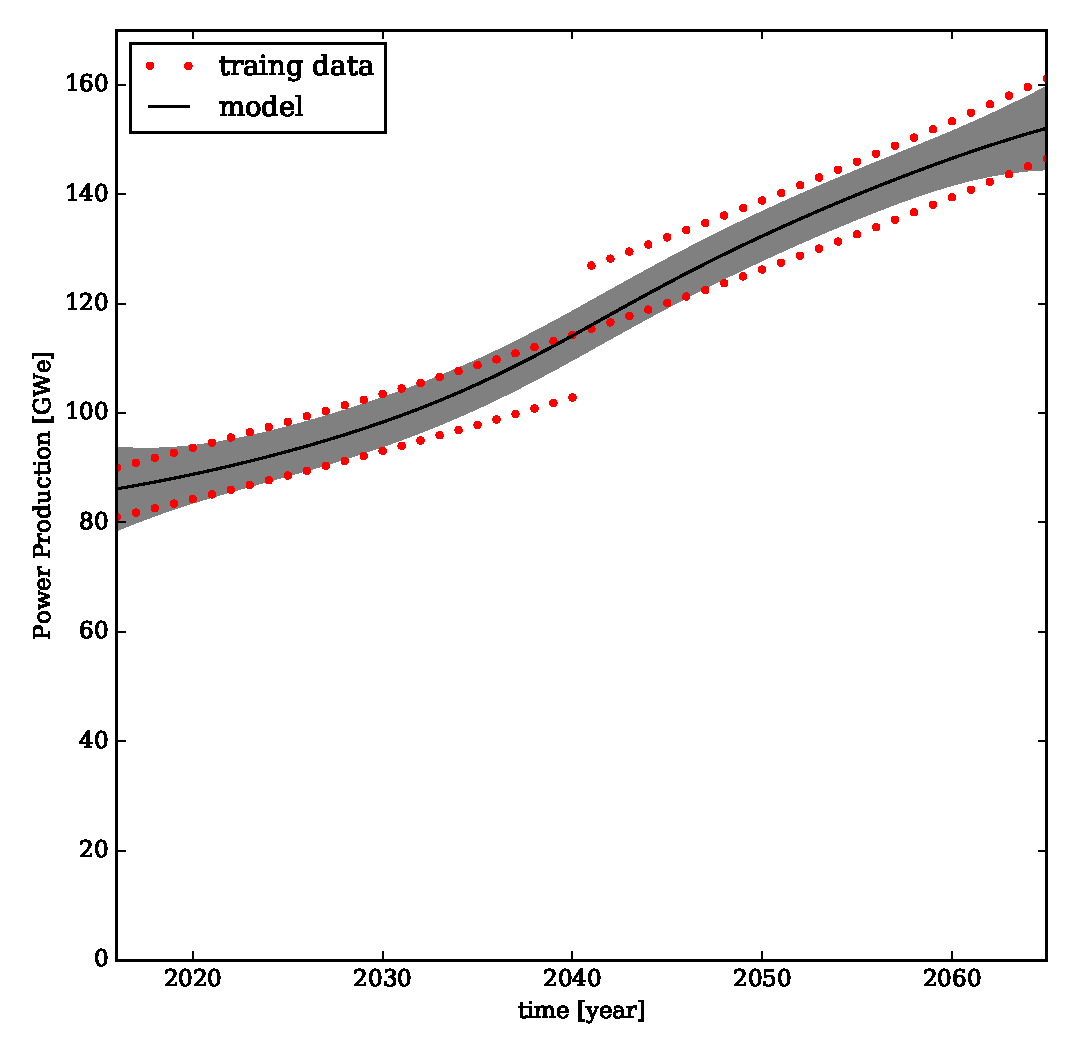
\includegraphics[width=0.9\textwidth]{gwe-model-.eps}
\caption{The Gaussian process model of a 1\% growth curve along with the
an inital 10\% under production followed by a 10\% under production. 
The model is represented by the black line that runs between the red 
training points. Two standard deviations form the model are displayed as the
gray region.}
\label{gwe-model-}
\end{figure}

The simple example above does not take advanatage of an important 
feature of Gaussian processes. Namely, it is not limitied to two production
curves in the training set.  As many as desirable may be used.  This will
allow the WORG algorith to dynamically adjust the number of $Z$ simulations 
are used to predict the next deployment schedule. This allows WORG to 
effortlessly expand $Z$ when new, useful simulations yeild valuable production
curves.  However, it also allows $Z$ to contract to discard production
curves that would drive the deployment schedule away from an omptimum.

Now that the Gaussian process regression and dynamic time warping tools have 
been added to the toolbox, the architechure of the WORG algorithm can 
itself be examined.

\clearpage